\documentclass[10pt,a4paper]{article}
\usepackage[utf8]{inputenc}

\usepackage[landscape,margin=1cm]{geometry}
\usepackage[english]{babel}


% colour themes to come. KnitR?

%-------------------------

\title{Instructions for using RBTools for Mac}
\date{2019}
\usepackage[default]{raleway}
\usepackage{fontawesome}
\usepackage[T1]{fontenc}

\usepackage{hyperref}
\usepackage{enumitem}
\usepackage{lipsum}

\usepackage{xcolor}
\definecolor{customcolor}{HTML}{616AC5}
\definecolor{alert}{HTML}{CD5C5C}
\definecolor{w3schools}{HTML}{4CAF50}
\definecolor{subbox}{gray}{0.60}
\definecolor{codecolor}{HTML}{FFC300}
\colorlet{xx}{customcolor}


%--------------------------Editor mode.

\usepackage
[citestyle=authoryear,
sorting=nty,	  		%Sorts bibliography by year, name, title
autocite=footnote, 		%Autocite command generates footnotes
autolang=hyphen, 		
mincrossrefs=1, 	
backend=biber]
{biblatex}

\DeclareFieldFormat{postnote}{#1}
\DeclareFieldFormat{multipostnote}{#1}
\DeclareAutoCiteCommand{footnote}[f]{\footcite}{\footcites}

\bibliography{literature}
%----------------------------------------
%--------------------------------------------------------------------------------
\usepackage{tcolorbox}

\tcbuselibrary{most,listingsutf8,minted}

\tcbset{tcbox width=auto,left=1mm,top=1mm,bottom=1mm,
right=1mm,boxsep=1mm,middle=1pt}

\newenvironment{mycolorbox}[2]{%
\begin{tcolorbox}[grow to left by=-1em,grow to right by=-1em,capture=minipage,fonttitle=\large\bfseries, enhanced jigsaw,boxsep=1mm,colback=#1!30!white,on line,tcbox width=auto, toptitle=0mm,colframe=#1,opacityback=0.7,nobeforeafter,title=#2]%
}{\end{tcolorbox}\\[0.2em]}

\newenvironment{subbox}[2]{%
\begin{tcolorbox}[capture=minipage,fonttitle=\normalsize\bfseries, enhanced jigsaw,boxsep=1mm,colback=#1!30!white,on line,tcbox width=auto,left=0.3em,top=1mm, toptitle=0mm,colframe=#1,opacityback=0.7,nobeforeafter,title=#2]\footnotesize %
}{\normalsize\end{tcolorbox}\vspace{0.1em}}

\newenvironment{multibox}[1]{%
\begin{tcbraster}[raster columns=#1,raster equal height,nobeforeafter,raster column skip=1em,raster left skip=1em,raster right skip=1em]}{\end{tcbraster}}

\newenvironment{textbox}[1]{\begin{mycolorbox}{customcolor}{#1}}{\end{mycolorbox}}

%-------------------------------
\newtcblisting{codebox}[2]{colback=codecolor!5,colframe=codecolor!80!black,listing only, 
minted options={numbers=left,style=tcblatex,fontsize=\tiny,breaklines,autogobble,linenos,numbersep=3mm},
left=5mm,enhanced,
title=#2, fonttitle=\bfseries,
listing engine=minted,minted language=#1}

%--------------------------------------------------------------------------------
\newcommand{\punkti}{~\lbrack\dots\rbrack~}

\renewenvironment{quote}
               {\list{\faQuoteLeft\phantom{ }}{\rightmargin\leftmargin}%
                \item\relax\scriptsize\ignorespaces}
               {\unskip\unskip\phantom{xx}\faQuoteRight\endlist}
               

%--------------------------------------------------------------------------------
\newcommand{\bgupper}[3]{\colorbox{#1}{\color{#2}\huge\bfseries\MakeUppercase{#3}}}
\newcommand{\bg}[3]{\colorbox{#1}{\bfseries\color{#2}#3}}

\newcommand{\mycommand}[2]{{\ttfamily\detokenize{#1}}~\dotfill{}~{\footnotesize #2}\\}
\newcommand{\sep}{{\scriptsize~\faCircle{ }~}}


\newcommand{\bggreen}[1]{\medskip\bgupper{w3schools}{black}{#1}\\[0.5em]}
\newcommand{\green}[1]{\smallskip\bg{w3schools}{white}{#1}\\}
\newcommand{\red}[1]{\smallskip\bg{alert}{white}{#1}\\}

\usepackage{multicol}
\setlength{\columnsep}{30pt}

\setlength{\parindent}{0pt}
\pagestyle{empty}

\usepackage{csquotes}

\newcommand{\loremipsum}{Lorem ipsum dolor sit amet.}



%--------------------------------------------------------------------------------
\begin{document}
\small

\maketitle
\thispagestyle{empty}
\scriptsize
\tableofcontents



\newpage

%--------------------------------------------------------------
\section{Tools}

The RBTools for Mac package uses three main tools: Zotero, Hypothes.is and Open Semantic Search

\vspace{0.5cm}

\begin{textbox}{Zotero}
 \href{https://zotero.org}{Zotero} \sep \href{https://zotero.org}{bibliographic software}

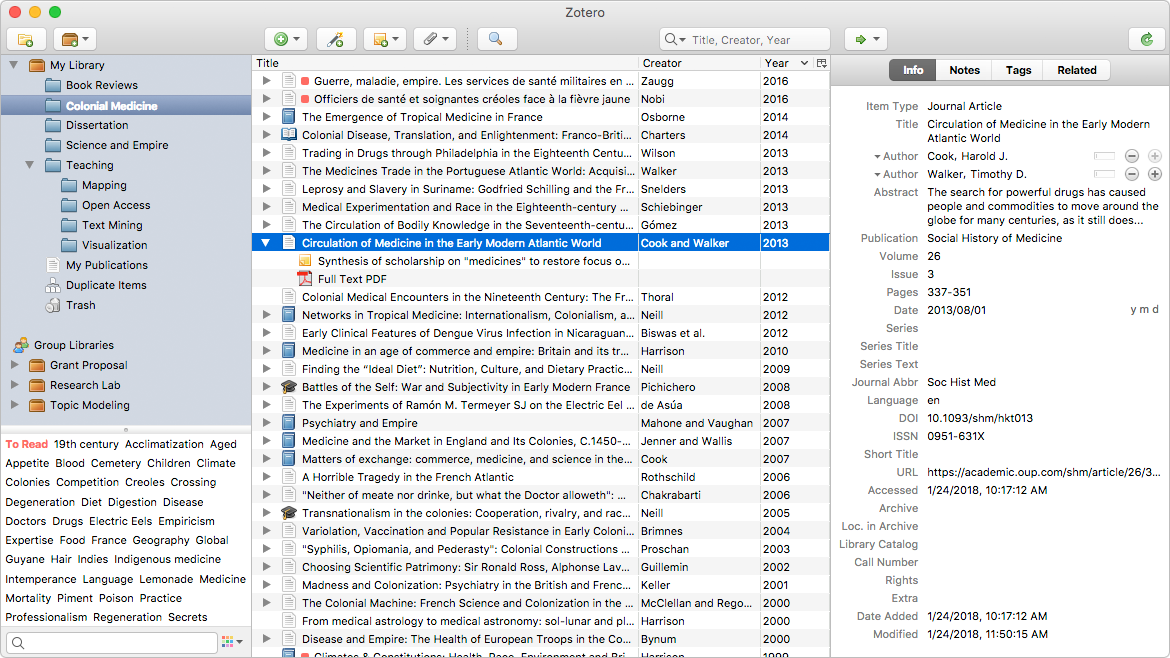
\includegraphics[width=\textwidth]{zotero.png}
\end{textbox}

\begin{textbox}{Hypothes.is}
 \href{https://hypothes.is/}{Hypothes.is} \sep \href{https://hypothes.is/}{Web annotation}

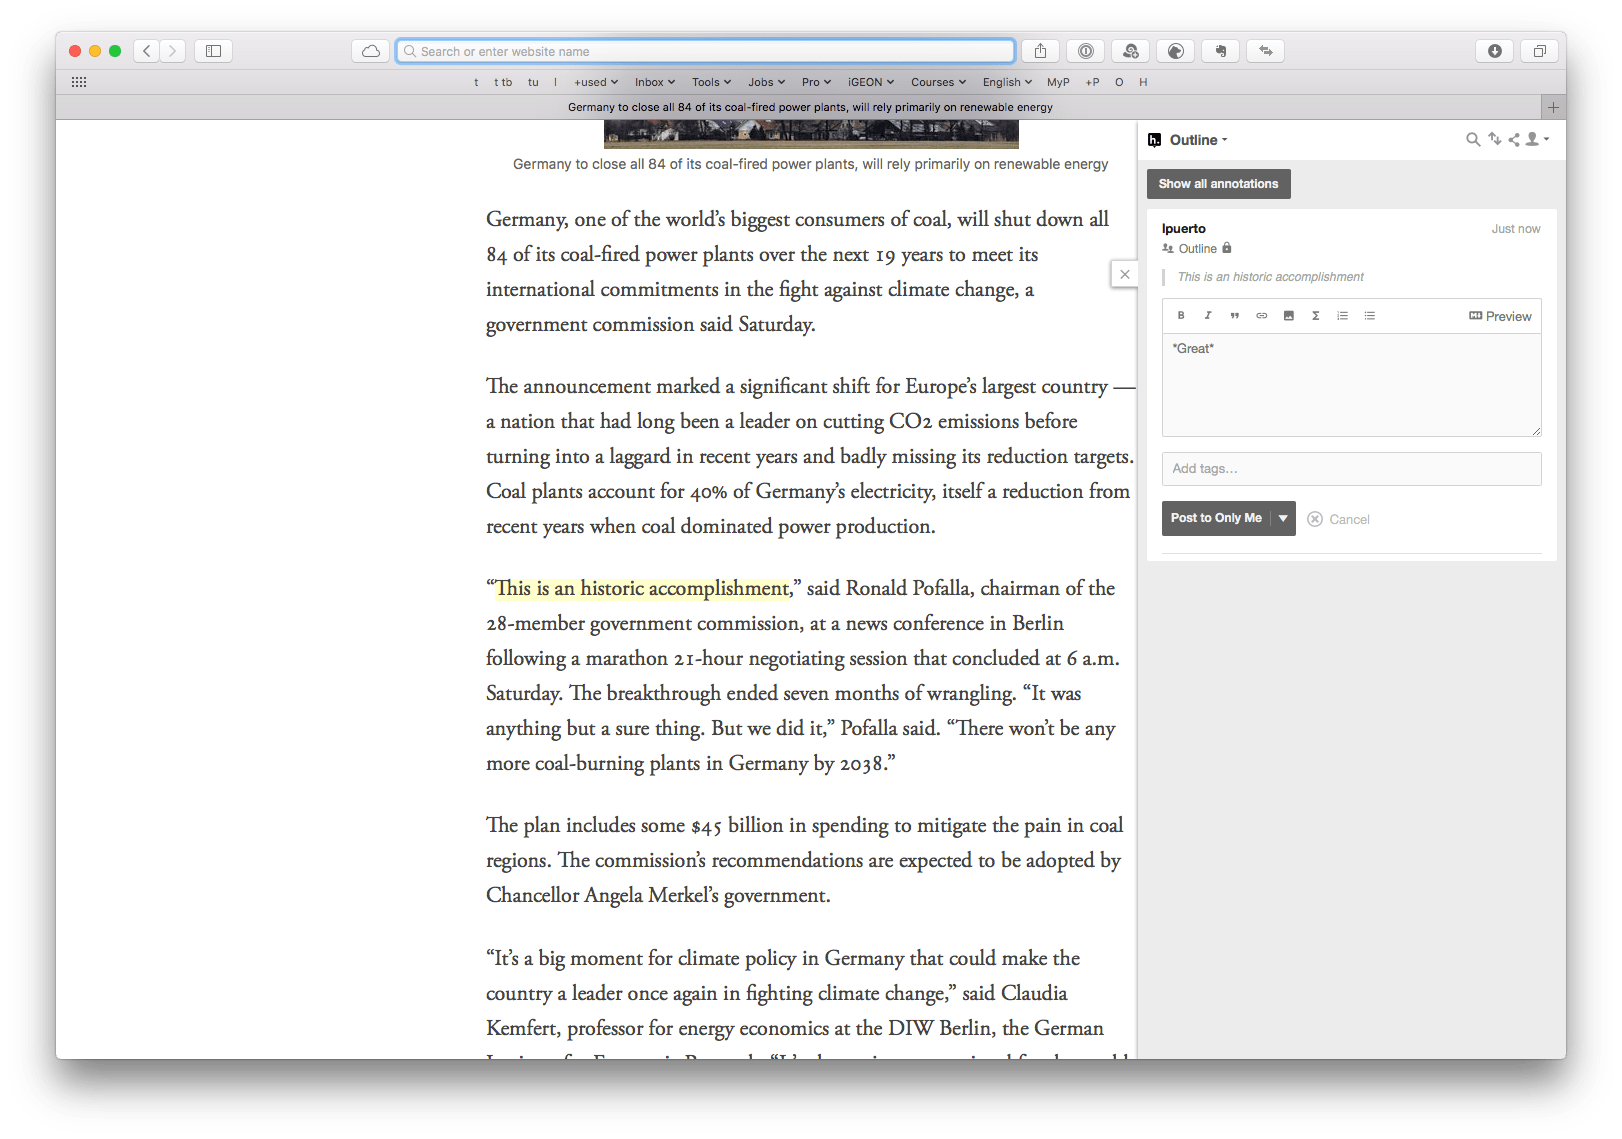
\includegraphics[width=\textwidth]{Hypothesis.png}

\end{textbox}

\begin{textbox}{Open Semantic Search}
\href{https://www.opensemanticsearch.org}{Open Semantic Search} \sep \href{https://www.opensemanticsearch.org}{Search Engine and Open Source Text Mining & Text Analytics}

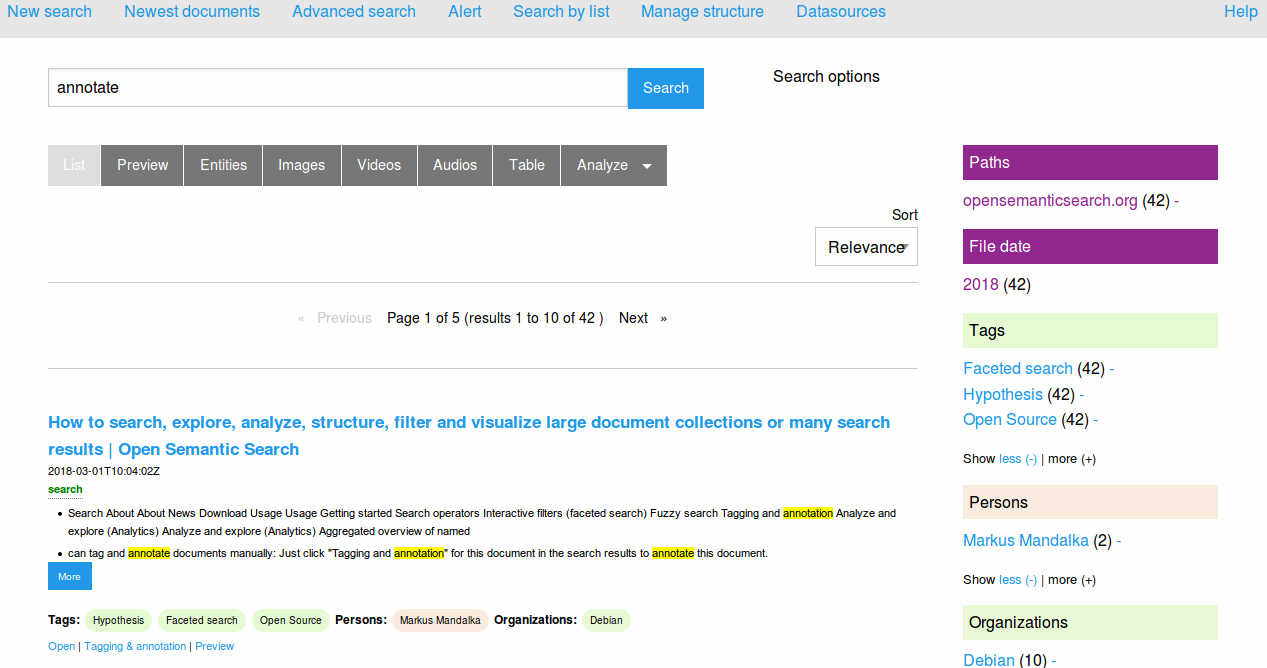
\includegraphics[width=\textwidth]{search.png}

\end{textbox}


%--------------------------------------------------------------

\section{Getting Started}



\begin{textbox}{Install Package}
 

  

\green{Instructions}
\red{Package}
\begin{enumerate}
\item \textbf{Confirm} Operating System and disk space requirements are met by looking at readme.md in the Git repository.
\item \textbf{Download} from the repository at \href{https://github.com/MQ-FOAR705/Osmond-Chiu---Proof-of-Concept---Implementation.git}{https://github.com/MQ-FOAR705/Osmond-Chiu---Proof-of-Concept---Implementation.git}.
\item \textbf{Open} Zip File.
\item \textbf{Control}-click the RBTools package in unzipped folder then select open to begin installation and bypass any security settings that may prevent the file from running
\item \textbf{Read} the Readme.md file.
\item \textbf{Read} these instructions.
\item \textbf{Tick} off completed tasks from checklist.
\end{enumerate}

\end{textbox}

%--------------------------------------------------------------


\section{Zotero}
\subsection{Setup}
\begin{textbox}{Complete Installation}
 

  

\green{Instructions}
\red{Zotero}
\begin{enumerate}
\item \textbf{Check} that Zotero installation file has been mounted if installation does not automatically pop-up.
\item \textbf{Drag} the Zotero icon to 'Drag here to install'.
\item \textbf{Complete} Zotero installation.
\end{enumerate}

\end{textbox}

\begin{textbox}{Create account}
 

  

\green{Instructions}
\red{Zotero}
\begin{enumerate}
\item \textbf{Open} browser.
\item \textbf{Go to}  \href{https://www.zotero.org/user/login}{https://www.zotero.org/user/login} .
\item \textbf{Click} Register for a Free Account.
\item \textbf{Choose} the username and email address you want to use for the account.
\item \textbf{Click} Register and you’ll receive a confirmation email shortly.
\item \textbf{Click} on the link in the confirmation email you receive to confirm your account set up.
\end{enumerate}

\end{textbox}


\begin{textbox}{Sync account}
 

  

\green{Instructions}
\red{Zotero}
\begin{enumerate}
\item \textbf{Open} Zotero.
\item \textbf{Open} Preferences (via the Zotero menu) and select the Sync tab.
\item \textbf {Enter} your Zotero user name and password.
\item \textbf {Click} set up syncing.
\item \textbf {Check} both boxes under File Syncing and choose Zotero storage for My Library.
\item \textbf {Close} Preferences.
\item \textbf {Click} the green circular arrow button at the top right corner of the Zotero program window to sync account with software.
\end{enumerate}

\end{textbox}

\subsection{Using Zotero With Other Programs}

\begin{textbox}{Link Zotero to Overleaf}
 

  

\green{Instructions}
\red{Zotero}
\red{Overleaf}
\begin{enumerate}
\item \textbf{Open} Zotero
\item \textbf{Open} Preferences (via the Zotero menu) and select the Sync tab.
\item \textbf {Enter} your Zotero user name and password.
\item \textbf {Close} Preferences.
\item \textbf {Click} the green circular arrow button at the top right corner of the Zotero program window to sync account with software.
\item \textbf{Go to}  \href{https://www.overleaf.com/}{https://www.overleaf.com/}. 
\item \textbf{Register} an Overleaf account if you do not already have one.
\item \textbf {Log} into Overleaf
\item \textbf {Click} on Account then Account Settings.
\item \textbf {Scroll} down the page to Zotero Integration.
\item \textbf {Click} on 'Link to Zotero' and you will be prompted to log into Zotero.org
\item \textbf {Enter} Zotero username and password.
\item \textbf {Create} a New Private Key.
\item \textbf {Click} on Accept Defaults and you will be automatically returned to your Overleaf account settings page.
\item \textbf {Scroll} down to the bottom of the page to check Zotero Integration.
\end{enumerate}

\end{textbox}

 
 \begin{textbox}{Import references}
 

  

\green{Instructions}
\red{Zotero}
\red{Overleaf}
\begin{enumerate}
\item \textbf {Go} to Overleaf. 
\item \textbf {Select} the project that you want to link to Zotero.
\item \textbf {Select} New File from the top menu.
\item \textbf {Select} 'From Zotero', name the file for the project and choose a format (BibLaTeX).
\item \textbf {Go} to main.tex file and add your Zotero file (as a bib resource) to header with the codes \begin{verbatim} \usepackage{biblatex} and \bibliography{name_of_file.bib}\end{verbatim}.
\end{enumerate}

\end{textbox}

  

  \begin{textbox}{Insert references}
 

  

\green{Instructions}
\red{Zotero}
\red{Overleaf}
\begin{enumerate}
\item \textbf {Select} where you want to place the reference in the text.
\item \textbf {Write} /cite{} then enter in citation.
\end{enumerate}

\end{textbox}

  

 \begin{textbox}{Generate bibliography}
 

  

\green{Instructions}
\red{Zotero}
\red{Overleaf}
\begin{enumerate}
\item \textbf {Select} where you want to place the bibliography in the text.
\item \textbf{Insert} your bibliography by typing into the source code \begin{verbatim}/printbibliography\end{verbatim}.
\end{enumerate}

\end{textbox}


%--------------------------------------------------------------


\section{Hypothes.is}
\subsection{Setup}

\begin{textbox}{Create account}
 

  

\green{Instructions}
\red{Hypothes.is}
\begin{enumerate}
\item \textbf{Open} browser
\item \textbf{Go to} \href{hypothes.is/signup}{hypothes.is/signup}. 
\item \textbf{Choose} a username, enter your email address, and create a password.
\item \textbf{Click} Sign Up and you will receive a confirmation email to active your account.
\item \textbf{Click} the link in the email received to validate your email and activate your Hypothes.is account.
\end{enumerate}

\end{textbox}

\begin{textbox}{Add Chrome Extension}
 

  

\green{Instructions}
\red{Hypothes.is}
\begin{enumerate}
\item \textbf{Go to} web.hypothes.is/start. 
\item \textbf{Click} add-on for Chrome.
\item \textbf{Accept} the prompt in the pop up window to install the extension. 
\item \textbf{Consider} adding a bookmarklet if you do not have/use Chrome.
\end{enumerate}

\end{textbox}

\begin{textbox}{Add Bookmarklet}
 

  

\green{Instructions}
\red{Hypothes.is}
\begin{enumerate}
\item \textbf{Go to} web.hypothes.is/start. 
\item \textbf{Drag} 'Hypothesis Bookmarklet' to the bookmarks bar, or right-click/control-click to bookmark the link.
\end{enumerate}

\end{textbox}

\subsection{Using Hypothes.is}

\begin{textbox}{Create tag hierarchy}
 

  

\green{Instructions}
\red{Hypothes.is}
\begin{enumerate}
\item \textbf{Identify} what you want tagged based on topics, themes, keywords, source types. 
\item \textbf{Create} a text document to list tags.
\item \textbf{Write} down list of tags based on identified subjects.
\end{enumerate}

\end{textbox}


\begin{textbox}{Highlight}
 

  

\green{Instructions}
\red{Hypothes.is}
\begin{enumerate}
\item \textbf{Go to} webpage or open a local file in a browser to highlight. 
\item \textbf{Click} on Hypothes.is icon in browser toolbar or bookmarklet.
\item \textbf{Click} toggle or resize sidebar.
\item \textbf{Log} into your Hypothes.is account.
\item \textbf{Choose} whether you want the highlight to be public or in a private group.
\item \textbf{Select} text that you wish to highlight.
\item \textbf{Click} on the Highlight icon that appeals.

\end{enumerate}

\end{textbox}

\begin{textbox}{Annotate}
 

  

\green{Instructions}
\red{Hypothes.is}
\begin{enumerate}
\item \textbf{Go to} webpage or open a local file in a browser to annotate. 
\item \textbf{Click} on Hypothes.is icon in browser toolbar or bookmarklet.
\item \textbf{Click} toggle or resize sidebar.
\item \textbf{Log} into your Hypothes.is account.
\item \textbf{Choose} whether you want the highlight to be public or in a private group.
\item \textbf{Select} text that you wish to annotate.
\item \textbf{Click} on the Annotate icon that appeals.
\item \textbf{Type} annotations in text box.
\item \textbf{Type} tags for the annotation.
\item \textbf{Choose} where to post the annotations (public or private group) and click. 

\end{enumerate}

\end{textbox}


\begin{textbox}{Generate API token}
 

  

\green{Instructions}
\red{Hypothes.is}
\begin{enumerate}
\item \textbf{Go to} Hypothes.is website. 
\item \textbf{Log} into your Hypothes.is account.
\item \textbf{Click} on gear icon.
\item \textbf{Click} on 'Developer.
\item \textbf{Click} Generate Your API token.
\item \textbf{Copy} token in text box for use.

\end{enumerate}

\end{textbox}


\section{Open Semantic Search}
\subsection{Setup}


\begin{textbox}{Install VirtualBox}
 

  

\green{Instructions}\red{Open Semantic Search}

\begin{enumerate}
\item \textbf {Double-click} on the VirtualBox.pkg installer file displayed in Install-Package folder on Desktop.
\item \textbf {Select} where to install Oracle VM VirtualBox.

\end{enumerate}


\end{textbox}

\begin{textbox}{Install Open Semantic Search}
 

  

\green{Instructions}\red{Open Semantic Search}
\begin{enumerate}
\item \textbf{Download} the virtual machine image Open Semantic Desktop Search. 
\item \textbf {Find} Oracle VM VirtualBox icon in the "Applications" folder in the Finder.
\item \textbf{Start} VirtualBox.
\item \textbf{Go} into the menu "File" start the option "Import Appliance".
\item \textbf{Click} folder icon then choose the Open Semantic Desktop Search .ova file and select "Continue"
\item \textbf{Click} "Import" at the bottom of the pop-up screen.
\item \textbf{Edit} the settings of the new virtual machine (choose the virtual machine in the left sidebar and click the Settings button in the top bar).
\item \textbf{Go} to "Shared Folders" then click the Add Shared Folders icon.
\item \textbf{Click} on "Folder Path" then select folder.
\item \textbf{Activate} the option Auto-mount then click "Ok".
\end{enumerate}

\end{textbox}

\subsection{Using Open Semantic Search}

\begin{textbox}{Load Open Semantic Search}
 

  

\green{Instructions}\red{Open Semantic Search}
\begin{enumerate}
\item \textbf{Start} VirtualBox if not open yet.
\item \textbf{Select} Open Semantic Desktop Search.
\item \textbf{Click} on Start Icon. 
\end{enumerate}

\end{textbox}


\begin{textbox}{Text search}
 
  

\green{Instructions}\red{Open Semantic Search}
\begin{enumerate}
\item \textbf{Enter} text into the Open Semantic Search interface. 
\item \textbf{Click} search.
\item \textbf{Select} relevant filter in facets on the right navigation sidebar. 
\end{enumerate}

\end{textbox}


\begin{textbox}{Create tags}
 

  

\green{Instructions}\red{Open Semantic Search}
\begin{enumerate}
\item \textbf{Click} on Thesaurus in the topbar of the Open Semantic Search interface.
\item \textbf{Select} Tag as Facet. 
\item \textbf{Open} file with list of tags (if using existing tag)
\item \textbf{Type} name of tag.
\item \textbf{Type} name of tag into file with list of tags if not existing and save.
\item \textbf{Save} tag. 
 
\end{enumerate}

\end{textbox}

\begin{textbox}{Tag documents}

  

\green{Instructions}
\red{Open Semantic Search}
\begin{enumerate}
\item \textbf{Search} for document you wish to tag.
\item \textbf{Click} Tagging and annotation for this document in the search results.
\item \textbf{Add} the pre-existing tags to the document. 
\end{enumerate}

\end{textbox}


\begin{textbox}{Import from Hypothes.is}

  

\green{Instructions}\red{Open Semantic Search}\red{Hypothes.is}
\begin{enumerate}
\item \textbf{Repeat} previous instructions to find API token in Hypothes.is account. 
\item \textbf{Don't} regenerate a new token.
\item \textbf{Copy} API Token.
\item \textbf{Open} loaded Open Semantic Search.
\item \textbf{Click} on Datasources in the topbar of the Open Semantic Search interface.
\item \textbf{Click} on Annotations (Hypothesis).
\item \textbf{Enter} copied API Token for Authorization.
\end{enumerate}


\end{textbox}

\end{document}
















